\newpage

\notebox{\textbf{About the formatting of this document}: \mono{Monospace} text refers to a package, command, programming language or other programming-related concept. Text in {\color{glossary}green} refers to an entry in the glossary. Text in {\color{urlblue}this blue} is a link to an external source. Text in {\color{exturlblue}this blue} is a link to a section inside this document. Square brackets with {\color{citations}violet numbers} are citations.}

\importantbox{This document covers \mono{GATTACA} version \mono{0.3.2}.}

\newpage

\section{Introduction}

A common wish for a researcher in the genomics field is to compare the gene expression\footnote{More formally, the amount of mRNA in the sample, which often correlates directly with the amount of expressed protein.} of two (or more) different samples and obtain a list of \glspl{deg}. This procedure is known as \gls{dea}, and involves four steps: obtaining gene expression data, data preprocessing, running \gls{dea}, and annotation.

A - now almost obsolete - method of obtaining gene expression data is the usage of \textbf{microarrays}. Microarrays are solid chips upon which DNA probes are linked. mRNA is extracted from the samples, purified, amplified and retrotranscribed to cDNA. The resulting \glspl{library} are then applied on the chips. The probes will link to complementary sequences, and, after washing and using specific imaging methods, the amount of linkage for each probe can be detected. The resulting intensities are directly correlated with the expression of the mRNA in the samples.

Raw intensity data from microarry scanners (henceforth "raw data") needs to be preprocessed before \glspl{deg} can be detected. In the context of this document, we define "\gls{mdp}" as the set of steps that need to be performed on such data to obtain an \textbf{expression dataset}. An expression dataset is a matrix with columns representing different samples (microarrays) and rows representing genes detected by the microarrays. The values in the matrix represent the \mono{log2} expression values for that gene/sample combo.
\gls{mdp} is a multi-step, platform-dependent process. Many packages are available in the \mono{R} programming language to perform \gls{mdp}, for example \mono{limma} \cite{ritchieLimmaPowersDifferential2015}, \mono{oligo}, and \mono{affycoretools}. Knowledge of \mono{R} is needed to use these tools.

One of the most widely known and used tools to perform \gls{dea} is \mono{limma}, which uses (generalized) linear models to detect \glspl{deg}. \mono{RankProd} is another package that can detect \glspl{deg} using non-parametric, rank-based approaches \cite{hongRankProdBioconductorPackage2006}. Both these packages are implemented in the \mono{R} language, and require some knowledge of \mono{R} to be used.

Finally, microarray scanners will label the intensities with their respective probe IDs, while an human researcher prefers Gene Symbols (or \gls{hugo} symbols). This step is called \textit{annotation}, and requires the use of one of many annotation databases that hold the correspondences between probe IDs and Gene Symbols, among other.

There is currently a need for a simple tool that can analyse microarray expression data to produce a list of \glspl{deg} using an intuitive, user friendly interface. We present \gls{gattaca}, a self-contained tool to prepare, analyse and annotate microarray gene expression data. An additional benefit of \gls{gattaca} is its reproducibility. Being containerized, the tool is guaranteed to be computationally reproducible.

One of the strengths of \gls{gattaca} is its user friendliness, so that any researcher, even without a background in bioinformatics or knowledge of \mono{R}, can correctly analyze both novel and pre-existing datasets.

\gls{gattaca} is written in \mono{R}, containerized in Docker and fully Open-Source. The source code is \href{https://github.com/Feat-FeAR/GATTACA}{hosted on GitHub}. Users are encouraged to propose enhancements and report issues on the website. \gls{gattaca} runs only on unix-like operating systems.

\subsection{Installation}
To install the tool, install \mono{Docker} (following \href{https://docs.docker.com/get-docker/}{the official guides}) and \mono{curl} (with your distribution's package manager of choice). Move into the folder where you'd like to install the tool, then run:

\begin{lstlisting}[style=ShellStyle]
curl https://raw.githubusercontent.com/Feat-FeAR/GATTACA/main/GATTACA --output GATTACA \
&& chmod +x ./GATTACA
\end{lstlisting}

Assuming that the folder where the script is placed is in your \mono{PATH}, the tool can be called with the \mono{GATTACA} command. This may be tested by running \mono{GATTACA --help}. If the command resolves with no errors, the tool is installed correctly.

\section{General options}
\gls{gattaca} can be called in the following way:
\begin{lstlisting}[style=ShellStyle]
GATTACA [-h | --help] [-v | --version <version>] [-l | --log_name <name>] <command> [<args>]
\end{lstlisting}

\begin{itemize}
    \item The \mono{-h | --help} flag ends the command early and prints a help message;
    \item The \mono{-v | --version <version>} optional parameter specifies the version of the docker to run. To see a list of the available containers, refer to the \href{https://github.com/Feat-FeAR/GATTACA/releases}{Github release page}. If unset, the \mono{latest} docker release is used instead.
    \item The \mono{-l | --log\_name <name>} parameter specifies the filename of the log file that is always created in the output folder. If unset, the filename is generated with the current date and time, and is therefore unique for each run.
\end{itemize}

The following sections describe the possible \mono{command}s and their respective \mono{args}.

\section{Data Preparation}

To prepare data from the raw files produced by the microarray scanning apparatuses (either \mono{.CEL} files for Affymetrix microarrays or \mono{.txt} files for Agilent), you can use the \mono{prepaffy} and \mono{prepagil} commands, which preprocess Affymetrix and Agilent data, respectively.

The commands are called as follows. For \mono{prepaffy}:
\begin{lstlisting}[style=ShellStyle]
GATTACA prepaffy [-h | --help] [-r | --remove-controls]
    [--plot-size <x,y>] [--png] [--plot-number <int>]
    <input_dir> <output_file>
\end{lstlisting}

\begin{itemize}
    \item The \mono{-h | --help} flag ends the command early and prints a help message;
    \item The \mono{-r | --remove-controls} flag, if set, causes the tool to filter out the control probes from the dataset. \gls{gattaca} does not give any other opportunity to do this.
    \item The \mono{--plot-size <x,y>}, \mono{--png} and \mono{--plot-number <int>} flag can be used to customize the behaviour of plotting. \mono{plot-size} controls the size of plots. If set, the \mono{--png} flag causes the plots to be printed as \mono{.png} format, and not the default of \mono{.pdf}. The tool prints one plot per input file. The \mono{plot-number} flag can limit the number of plots to \mono{<int>}.
    \item \mono{<input\_dir>} must be replaced with the (full) path to the input folder.
    \item \mono{<output\_file>} must be replaced with the (full) path to the file that will be written with the expression data. The file will be formatted according to the \mono{.csv} standard.
\end{itemize}

For \mono{prepagil}:
\begin{lstlisting}[style=ShellStyle]
GATTACA prepagil [-h | --help] [-r | --remove-controls]
    [-p | --grep-pattern <pattern>]
    [--plot-size <x,y>] [--png] [--plot-number <int>]
    <input\_dir> <output\_file>
\end{lstlisting}

For the \mono{-h | --help}, \mono{-r | --remove-controls}, \mono{--plot-size <x,y>}, \mono{--png} and \mono{--plot-number <int>} flags, refer to the definitions above. The same applies for the \mono{<input\_dir>} and \mono{<output\_file>} arguments.
\begin{itemize}
    \item The optional flag \mono{-p | --grep-pattern <pattern>} overrides the default detection for the Agilent input files from \mono{*.txt} to \mono{<pattern>} (see the detailed descriptions below).
\end{itemize}

Both commands perform the following steps:
\begin{enumerate}
    \item Find and load all input files;
    \begin{itemize}
        \item \mono{prepaffy} finds all files ending with the \mono{.CEL} file extension in the target folder, and considers them as input. \mono{prepagil}, instead, finds by default all \mono{.txt} files. This can be customized in the call, however, as \mono{.txt} is a common file extension.
    \end{itemize}
    \item Merge all inputs into a single expression file;
    \begin{itemize}
        \item Both commands do this automatically, by collapsing probes referring to the same gene (the so-called "probe-set") to a single entry.
    \end{itemize}
    \item Make MA plots before normalization, as well as an overall expression boxplot  (see section \ref{sec:QCplots} for more information about the quality control plots);
    \item Normalize the expression data;
    \begin{itemize}
        \item The \mono{prepaffy} command uses the \gls{rma} procedure to normalize the data, while the \mono{prepagil} uses a combination of background normalization and interarray correction provided by the \mono{limma} package.
    \end{itemize}
    \item Make MA plots and an expression boxplot after the normalization, allowing to appreciate the effects of normalization;
    \item If specified, remove control probes from the dataset;
    \item \mono{prepagil} collapses replicate probes by taking their mean value inside each sample;
    \item The final datasets are saved to the output file.
\end{enumerate}

The resulting file is ready to be analyzed by the other \gls{gattaca} commands, such as \mono{run} or \mono{annotate}.

\section{Differential Gene Expression Analysis}
The core functionality of \gls{gattaca} is to handle performing \glspl{dea} with a user friendly interface. Note that for very complex analyses it could be better to use \gls{gattaca} locally, by overriding some analysis steps. Refer to section \ref{localGATTA} for more information.

The steps to take to perform a \gls{dea} with \gls{gattaca} are as follows:
\begin{enumerate}
    \item Make a configuration file for the run;
    \item Edit the configuration file to customize it to the required experimental design;
    \item Run \mono{gattaca run}.
\end{enumerate}

In the following sections we explore how to execute these steps.

\subsection{Create a config file}
To create a configuration file, use the \mono{gattaca init} command:
\begin{lstlisting}[style=ShellStyle]
GATTACA init [-h | --help] <file_path>
\end{lstlisting}
Replace \mono{<file\_path>} with the (full) file path to where the config file should be created. The contents of the file may be changed at will.

\subsection{Customize the config file}
The configuration file created in the previous step follows the \mono{yaml} format, whose specifications may be seen at the \href{https://yaml.org/}{official \mono{yaml} website}\footnote{At the time of writing, the latest specification is \mono{yaml 1.2.2}}. A mini guide to \mono{yaml} is available in section \ref{miniyamlguide}.

The options are divided into sections. Each section controls different aspects of the analysis. The possible types of the various options are annotated in parentheses. The options available in \gls{gattaca} are:

\begin{itemize}
    \item \textbf{\mono{general}}: The general section contains general options to control plot size and type, whether to include annotations, and if to print extra data snippets during the analysis:
    \begin{itemize}
        \item \textbf{\mono{slowmode} (\mono{bool})}: If \mono{true}, asks for confirmation after every analysis step. The default is \mono{false}.
        \item \textbf{\mono{show\_data\_snippets} (\mono{bool})}: If \mono{true}, prints extra snippets of data during the analysis. This is useful together with \mono{slowmode} to see if the analysis is not doing anything wrong. The default is \mono{false}.
        \item \textbf{\mono{save\_pdf} (\mono{bool})}: If \mono{true}, saves plots in \mono{.pdf} format.
        \item \textbf{\mono{save\_png} (\mono{bool})}: If \mono{true}, saves plots in \mono{.png} format.
        \item \textbf{\mono{plot\_width} (\mono{int})}: The width of the plots, in inches.
        \item \textbf{\mono{plot\_height} (\mono{int})}: The height of the plots, in inches.
        \item \textbf{\mono{png\_resolution} (\mono{int})}: The pixels per inch of the png plots.
        \item \textbf{\mono{enumerate\_plots} (\mono{bool})}: If \mono{true}, each plot is marked with a number, in the order it is created.
        \item \textbf{\mono{annotation\_chip\_id} (\mono{str})}: The "chip id" string of the chip used to find the \gls{hugo} symbols of the respective probes. A table of the available chip ids can be seen in table \ref{tab:chipids}.
    \end{itemize}
    \item \textbf{\mono{switches}}: The switches section contains various parameters to turn parts of the analysis on or off:
    \begin{itemize}
        \item \textbf{\mono{dryrun} (\mono{bool})}: Run the analysis, but do not save any output plots (with the exception of the log file). This can be useful to test out the analysis before committing to it, especially when used in combination with the \mono{slowmode} and \mono{show\_data\_snippets} options.
        \item \textbf{\mono{renormalize} (\mono{bool})}: Run quantile-quantile normalization on the data. This can be useful to normalize "unruly" samples, for which the normalization steps in \mono{prepaffy} and \mono{prepagil} are not enough. Additional plots are saved to appreciate this extra normalization step.
        \item \textbf{\mono{limma} (\mono{bool})}: Run \gls{dea} with \mono{limma}.
        \item \textbf{\mono{rankproduct} (\mono{bool})}: Run \gls{dea} with \mono{RankProduct}.
    \end{itemize}
    \item \textbf{\mono{design}}: The design section contains crucial options to set the experimental design that will be used to steer the analysis.
    \begin{itemize}
        \item \textbf{\mono{experimental\_design} (\mono{str})}: The experimental design of the experiment. It must be a comma-delimited set of values, of the same length as the number of input samples, with each value being the label for the experimental variable of interest. Numbers specified at the end of each group can be used to represent sample pairings. For a detailed guide on how to define this parameter, see section \ref{exprdesign}.
        \item \textbf{\mono{contrasts} (\mono{list of str})}: A list of strings of the type \mono{"group1-group2"}, where each "group" is a level in the experimental design. Each value in the list specifies a (different) contrast of interest. For a detailed guide on how to define this parameter, see section \ref{exprdesign}.
        \item \textbf{\mono{batches} (\mono{null} OR \mono{str})}: If \mono{null}, no batch effect will be corrected, assuming all samples derive from the same batch. If \mono{str}, it is treated similar to the \mono{experimental\_design} string, and each level refers to a different batch. Note that \mono{RankProd} cannot correct batch effects if, inside each batch, there are not at least than two samples for each experimental condition.
        \item \textbf{\mono{extra\_limma\_vars} (\mono{null} OR \mono{list of str})}: If \mono{null}, nothing happens. If \mono{list of str}, each string in the list is treated similar to the \mono{experimental\_design} string, adding an additional variable to the \mono{limma} analysis. This can be useful to control for additional confounding variables in the experiment.
        \item \textbf{\mono{group\_colors} (\mono{list of str})}: A list of strings that can be understood by \mono{R} to be a colour. Each colour will be paired with a different condition type in the experimental design, so at least that many colours must be specified. A list of possible colours can be found \href{http://www.stat.columbia.edu/~tzheng/files/Rcolor.pdf}{here}.
        \item \textbf{\mono{filters}}: The parameters used by the analysis to filter the data:
        \begin{itemize}
            \item \textbf{\mono{log2\_expression} (\mono{float})}: Filter out any genes that have lower $\log_2$ expression than this value. This value depends a lot on the experiment, and is generally higher for Agilent arrays. The default of "4" is good for Affymetrix arrays.
            \item \textbf{\mono{fold\_change} (\mono{float})}: Filter out (mark as non-differentially-expressed) any genes that have lower absolute Fold Change than this value. This is used to remove from the analysis all genes that, even if detected to be \glspl{deg}, as additional validation with other methods (such as \mono{PCR}) would be impossible.
            \item \textbf{\mono{min\_groupwise\_presence} (\mono{float})}: A value between $0$ and $1$, representing the proportion of samples in a single group of interest in which the \mono{fold\_change} filter threshold must be violated to be filtered out. If a gene passes the filter in at least one group, it is retained in the analysis. This allows for a more conservative filtering of the genes.
        \end{itemize}
    \end{itemize}
\end{itemize}

\begin{table}
    \centering
    \begin{tabular}{|c|c|}
        \hline
        Chip ID & Microarray name \\ \hline
        \mono{hgu133a} & Affymetrix Human Genome U133 Set (A) \\
        \mono{hgu133b} & Affymetrix Human Genome U133 Set (B) \\
        \mono{hgu133plus2} & Affymetrix Human Genome HG-U133 Plus 2.0 Array \\
        \mono{HsAgilentDesign026652} & Agilent-026652 Whole Human Genome Microarray 4x44K v2 \\
        \mono{hugene10st} & Affymetrix Human Gene 1.0-ST Array \\
        \hline
    \end{tabular}
    \caption{Chip IDs and the corresponding microarrays. The chip id codes must be used instead of the longer names when using \gls{gattaca}.}
    \label{tab:chipids}
\end{table}

\subsection{Running GATTACA}
Once the options file is created and edited, the process of running \mono{gattaca} is simple:
\begin{lstlisting}[style=ShellStyle]
GATTACA run [-h | --help] <output_dir> <input_file> <options_file>
\end{lstlisting}

\begin{itemize}
    \item Specifying the \mono{-h | --help} command ends execution early, and prints usage information.
    \item \mono{<output\_dir>} must be replaced with the (full) path to the output directory of choice. Note that, since the docker instance is run as administrator, the final owner of the output folder will be the original one, regardless of whom started the command. Sub-folders are created in this path, so it is recommended to be empty.
    \item \mono{<input\_file>} must be replaced with the (full) path to the input file, a \mono{.csv} file with the expression data, such as one created with \mono{prepaffy} or \mono{prepagil}. This file has one column per sample, and one row per gene. An additional column, named \mono{probe\_id}, contains the probe ids of the respective row names.
    \item \mono{<options\_file>} must be replaced with the (full) path to the options file used by the analysis.
\end{itemize}

\subsection{Defining the experimental design}
\label{exprdesign}

Defining the experimental design can seem daunting at first. Here are provided some guidelines on how to specify the relevant parameters in the analysis.

\subsubsection{Design strings}
A "design string" is a \mono{string} that expresses the value of some categorical variable on each sample, with each variable separated by a comma (spaces are ignored). We will take as example four samples named "A", "B", "C" and "D", included in this order (from left to right) in an input file. Samples "A" and "C" are "control" samples, while samples "B" and "D" are "treated" samples. If we want to express this variable (the status of the samples) in a design string, we would write: \mono{"control, treated, control, treated"}.

Design strings can be very repetitive, and very long if many samples are present in the analysis. Two shorthands are provided to alleviate this:
\begin{itemize}
    \item \mono{"(...):x"}: Values (\mono{...}) in the parentheses are repeated sequentially "\mono{x}" number of times. For example: \mono{"(a, b):2"} is equal to \mono{"a, b, a, b"}.
    \item \mono{"[...]:x"}: Values (\mono{...}) in the parentheses are repeated each a "\mono{x}" number of times. For example: \mono{"[a, b]:2"} is equal to \mono{"a, a, b, b"}.
\end{itemize}

Please note that these patterns \textbf{cannot} be nested, but they can be used together (\mono{"(a, b):3, b, a, [a]:3, b"} is valid, for example). The same example from before can, therefore, be expressed with the equal string \mono{"(control, treated):2"} instead.

\subsubsection{The experimental design string}
The experimental design string, specified in \mono{design > experimental\_design}, represent the groups in which the samples fall in. These are the groups of interest for the analysis, and will be the same groups specified in the \mono{contrasts} parameter, determining between which samples \glspl{deg} have to be detected.

An additional variable that can be included in this same parameter is the sample pairings. Samples are paired if, for instance, they derive from the same patient, or the same tissue. This pairings can be expressed in the variable by adding a number, representing a certain pairing, at the end of each group name. For instance, consider six samples that fall into the "control" and "tumor" groups like such: \mono{"control, tumor, control, tumor, control, tumor"}. The first two samples come from the same patient, as do the next two and so on. This pairing can be expressed in the following way: \mono{"control1, tumor1, control2, tumor2, control3, tumor3"}. The actual numbers used are unimportant, as only the pairings of the samples are regarded.\\
The shorthand patterns support a way to specify these numbers automatically. By adding an asterisk (\mono{*}) at the end of the value, it will be replaced with a progressively increasing number automatically. For example, the string \mono{"control1, tumor1, control2, tumor2, control3, tumor3"} can be expressed as \mono{"(control*, tumor*):3"}. \mono{"[control*, tumor*]:2"} instead expands to \mono{"control1, control2, tumor1, tumor2"}. Note that any numbers that are already present in the string will be skipped by the shorthand patterns. For instance, \mono{"tumor4, (control*):2"} results is \mono{"tumor4, control5, control6"}.

\importantbox{As numbers represent pairings, the group names cannot contain any numbers (even not in the end of the value). Additionally, either all samples must have a pairing annotation, or none may. If annotated, each different pairing must show at least one sample for each group variable.}

\subsubsection{Specifying technical replicates}
Technical replicates are samples which are identical in all ways (experimental variables, batches, operator, etc...) and vary only due to different measurement runs. For instance, the same sample can be measured by several different chips to control technical variability.

Specifying them here will allow the analysis to take them into account. This allows for increased statistical power\footnote{Note that not setting this variable when some samples are technical replicates is pseudo-replication, and can invalidate the analysis results.}.

\subsubsection{Specifying batches}
Running the analysis in batches is often necessary, but introduces so-called \textit{batch effects}, static differences in the expression measures due to technical variables (such as the operator that ran the analysis, the hybridization and exposure times, etc...). Batch effects have been handled in different ways in the literature. \textcite{nygaardMethodsThatRemove2016} offers a review of the subject, and \gls{gattaca} follows the recommended guidelines. When running the \mono{limma} analysis, the data is corrected by TODO. When running \mono{RankProd}, the batch effects are taken into account in the algorithm itself. Note that \mono{RankProd} may only correct batch effects if for each grouping variable there are at least two samples in each batch.

The various batches can be specified with the \mono{design > batches} variable.

\subsubsection{Additional limma variables}

\mono{limma} can accept a virtually infinite amount of variables to control the tests. Extra variables may be submitted to \mono{limma} in the \mono{design > extra\_limma\_vars}, as a list of design strings, one string per additional variable.

\subsection{Interpreting results}
\gls{gattaca} outputs several files. Other than the quality control plots (whose meaning can be seen in section \ref{sec:QCplots}), \mono{gattaca run} produces the following files:
\begin{itemize}
    \item \mono{correspondence\_table.csv}: This file contains the correspondence between the original sample names (in the input files) and the new labels assigned by \gls{gattaca}, with the group names. It can be used to check the correspondence between the original samples and the experimental design vector.
    \item \mono{DEG tables}: For each tool and each contrast, one \glspl{deg} table file is created, named with the pattern \mono{<tool> - DEG Table <contrast>.csv}.
    \begin{itemize}
        \item The \mono{limma} \glspl{deg} tables have the following columns:
        \begin{itemize}
            \item \mono{probe\_id}: The probe id related to the other results;
            \item \mono{logFC}: The computed $\log_2$ fold-change between the contrasted groups;
            \item \mono{AveExpr}: The average expression considering all samples;
            \item \mono{t}: The t statistic of the contrast;
            \item \mono{P.Value}: The original P-value originated from the \mono{t} statistic;
            \item \mono{adj.P.Val}: The Benjamini-Hochberg adjusted p-value.
            \item \mono{B}: The B statistics represents how likely the gene is differentially expressed, in log-odds.
            \item \mono{markings}: The final marking of the gene, it being upregulated (\mono{1}), downregulated (\mono{-1}), or not differentially expressed (\mono{0}). This is computed from the adjusted P-value with an $\alpha = 0.05$, and the \mono{logFC}, taking in consideration the \mono{logfc} filter.
            \item \mono{SYMBOL}: If a chip is specified, the \mono{SYMBOL} column contains \gls{hugo} symbols of the respective probes.
        \end{itemize}
        \item The \mono{RankProd} \glspl{deg} tables have the following columns:
        \begin{itemize}
            \item \mono{probe\_id}: The probe id related to the other results;
            \item \mono{gene.index}: Arbitrary labelling of genes, set by RankProd before generating sample permutations;
            \item \mono{logFC}: The computed $\log_2$ fold-change between the contrasted groups;
            \item \mono{RP/Rsum.UP}: RankProd score for upregulated genes;
            \item \mono{pfp.UP}: \gls{pfp} for upregulated genes, treated similar to the \mono{limma} \mono{adj.P.Val}.
            \item \mono{P.value.UP}: P-value for upregulated genes, computed from the RankProd score.
            \item \mono{RP/Rsum.DOWN}: RankProd score for downregulated genes;
            \item \mono{pfp.DOWN}: \gls{pfp} for downregulated genes, treated similar to the \mono{limma} \mono{adj.P.Val}.
            \item \mono{P.value.DOWN}: P-value for downregulated genes, computed from the RankProd score.
            \item \mono{markings}: The final marking of the gene, it being upregulated (\mono{1}), downregulated (\mono{-1}), or not differentially expressed (\mono{0}). This is computed from the \gls{pfp} values with an $\alpha = 0.05$, and the \mono{logFC}, taking in consideration the \mono{logfc} filter. The \gls{pfp} values for upregulation are used for genes with positive \mono{logFC}, and vice-versa.
            \item \mono{AveExpr}: The average expression considering all samples;
            \item \mono{SYMBOL}: If a chip is specified, the \mono{SYMBOL} column contains \gls{hugo} symbols of the respective probes.
        \end{itemize}
    \end{itemize}
\end{itemize}

For most applications, the \mono{markings} column can be used to retrieve up- and down-regulated genes in each contrast for each tool. Comparisons of the number of genes detected by the two tools are available in the quality control plots.

\section{Annotating Results}
Investigators are often interested in annotating their results with metadata. \gls{gattaca} provides the \mono{annotate} command to annotate any \mono{.csv} file with a \mono{probe\_id} column with annotations from Bioconductor databases for each chip.

The command is invoked as such:
\begin{lstlisting}
GATTACA annotate [-h | --help] [-s | --select <selections>] <input_file>
                 <output_file> <chip_id>
\end{lstlisting}
\begin{itemize}
    \item The \mono{-h | --help} ends the command early and shows usage statistics.
    \item The \mono{-s | --select <selections>} option can be used to select the metadata to annotate. The possible variables that can sourced from most databases are \mono{ACCNUM}, \mono{CHR}, \mono{CHRLOC}, \mono{CHRLOCEND}, \mono{ENSEMBL}, \mono{ENTREZID}, \mono{ENZYME}, \mono{GENENAME}, \mono{GO}, \mono{MAP}, \mono{OMIM}, \mono{PATH}, \mono{PMID}, \mono{REFSEQ}, \mono{SYMBOL} and \mono{UNIPROT}.
    \item \mono{<input\_file>} must be replaced with the (full) path to the input \mono{.csv} file to annotate.
    \item \mono{<output\_file>} must be replaced with the (full) path to the output \mono{.csv} file.
    \item \mono{<chip\_id>} must be replaced with a valid chip id. The supported chips are available in Table \ref{tab:chipids}.
\end{itemize}

\section{Quality control plots}
\label{sec:QCplots}
This section provides explanations on how to interpret the quality control plots produced by the various commands, and additional details on how these are created.

\subsection{MA plots}
\label{plot:MA}
An MA plot is an application of the Bland-Altman plots for genomic data, where each gene is plotted as a point at M and A coordinates. The M coordinate for each gene is the log-ratio of the expression of that gene between two samples\footnote{When reading "Group 1 vs Group 2" it is assumed that the M value is calculated as $\log_2(Group 2) - \log_2(Group 1)$}. The A coordinate is the average expression of that gene in the two samples.\\
If one or both of the samples is instead a \textit{group} of samples, the M coordinate is instead calculated on the log-ratio of the \textit{groupwise median} of the expression of each gene is the sample groups. The "A" coordinate is the average expression between all the samples.\\
MA plots generated by \gls{gattaca} provide density shading, showing regions with gradually increasing point density from blue to red.

An example MA plot can be seen in Figure \ref{fig:PlatinumMAplot}, from a spike-in experiment. It is generally expected to see a large number of genes around low "A" values, with low M spread. These are generally low-expressed genes, of which M values are non-zero due to biological variability. Genes that have high A values but low M values (on the center-right of the plot) are housekeeping genes. Genes that have high absolute M values are putative \glspl{deg}.

The overall trend of the plot is shown with a \gls{gam} regression line, in red.

\begin{figure}
    \centering
    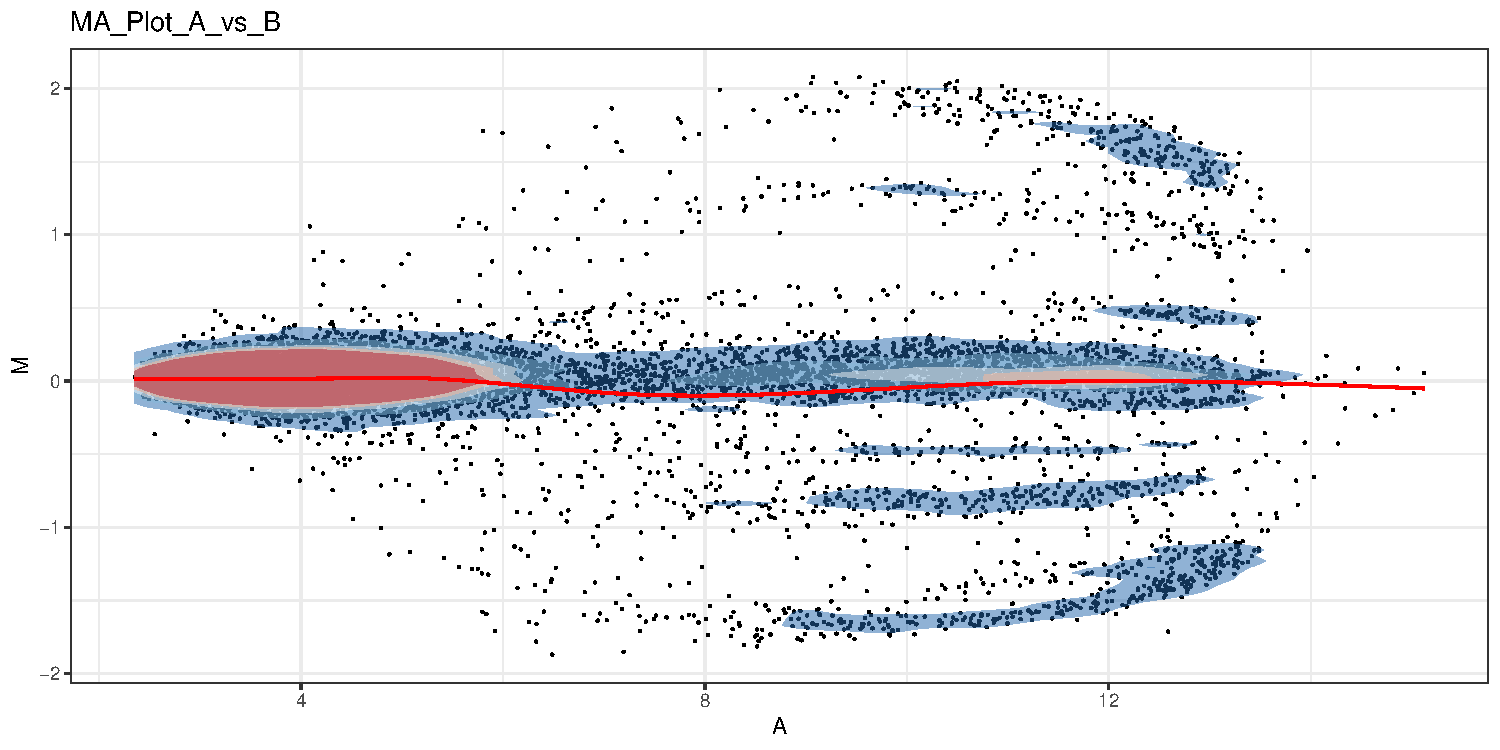
\includegraphics{resources/images/3_MA_Plot_A_vs_B.pdf}
    \caption{MA plot constructed with spike-in data from \textcite{zhuPreferredAnalysisMethods2010}. This MA plot shows the group of samples labelled as the "A" condition vs the group of samples labelled as the "B" condition.}
    \label{fig:PlatinumMAplot}
\end{figure}

We expect that MA plots for normalized data to be roughly linear and centered (as in, the \gls{gam} line flat and centered on zero). Both \mono{prepaffy}, \mono{prepagil} make one MA plot for each sample, plotting it versus the median expression of all other samples. When \mono{prepaffy} and \mono{prepagil} produce MA plots, they are ordered and numbered from the most distorted to the least, allowing the user to detect at a glance possibly distorted samples.

If a sample remains distorted after normalization, a possible mode of action is to remove it from the analysis. Otherwise, one may specify the \mono{renormalize} option in \mono{gattaca run} to perform quantile-quantile normalization on the data, forcing distorted samples to normality. Note however that doing this might also distort the results of the analysis.

The \mono{run} command also produces MA plots, with the purpose of highlighting differences between the groups of interest during \gls{dea}, as well as showing detected \glspl{deg} in a plot. An example of such an annotated plot is shown in Figure \ref{fig:PlatinumMAplotwithDEGs}

\begin{figure}
    \centering
    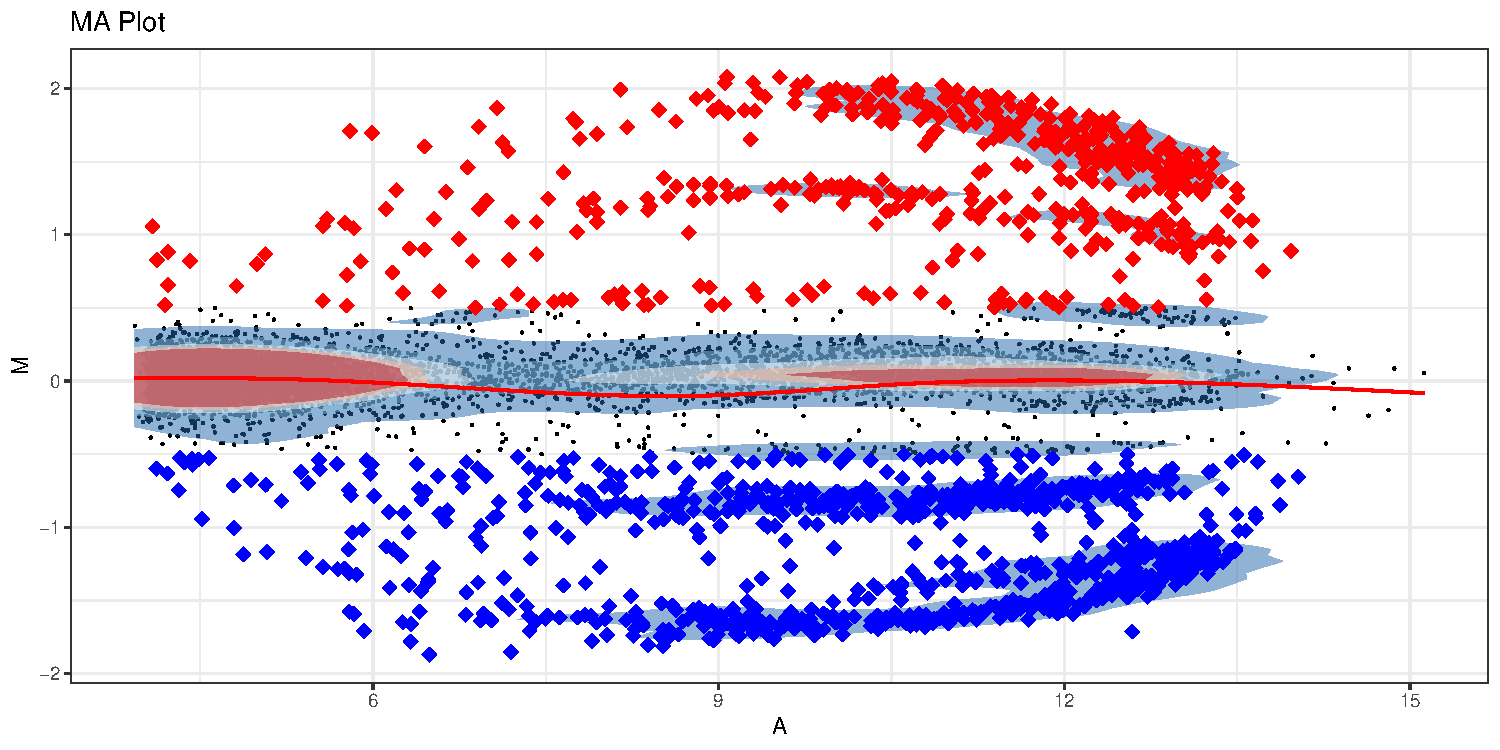
\includegraphics{resources/images/14_MA-Plot with Limma DEGs B-A.pdf}
    \caption{MA plots with added \glspl{deg} detected by the \mono{limma} package by comparing conditions "B-A". This plot was generated with the \mono{gattaca run} command on the spike-in Data from \textcite{zhuPreferredAnalysisMethods2010}. Genes highlighted in Red are detected to be significantly overexpressed in B in respect of A, while genes marked in Blue are similarly underexpressed in B in respect of A. That is, red-labelled genes are overexpressed \glspl{deg}, while blue-labelled genes are underexpressed \glspl{deg}.}
    \label{fig:PlatinumMAplotwithDEGs}
\end{figure}

\subsection{Expression Boxplots}
\label{plot:exprBox}
Each boxplot in an expression boxplot plot represents a different sample, with each point representing the expression value of each gene. An example of such a plot is shown in Figure \ref{fig:ExprBoxplot}. We expect that the general shape of all boxplots to be roughly similar, especially after normalization. If one or more samples have different shapes than the others, it is possible to employ the same procedures proposed in section \ref{plot:MA}: use the \mono{renormalize} option in \mono{gattaca run}, or eliminate the non-homogeneous sample(s).

\begin{figure}
    \centering
    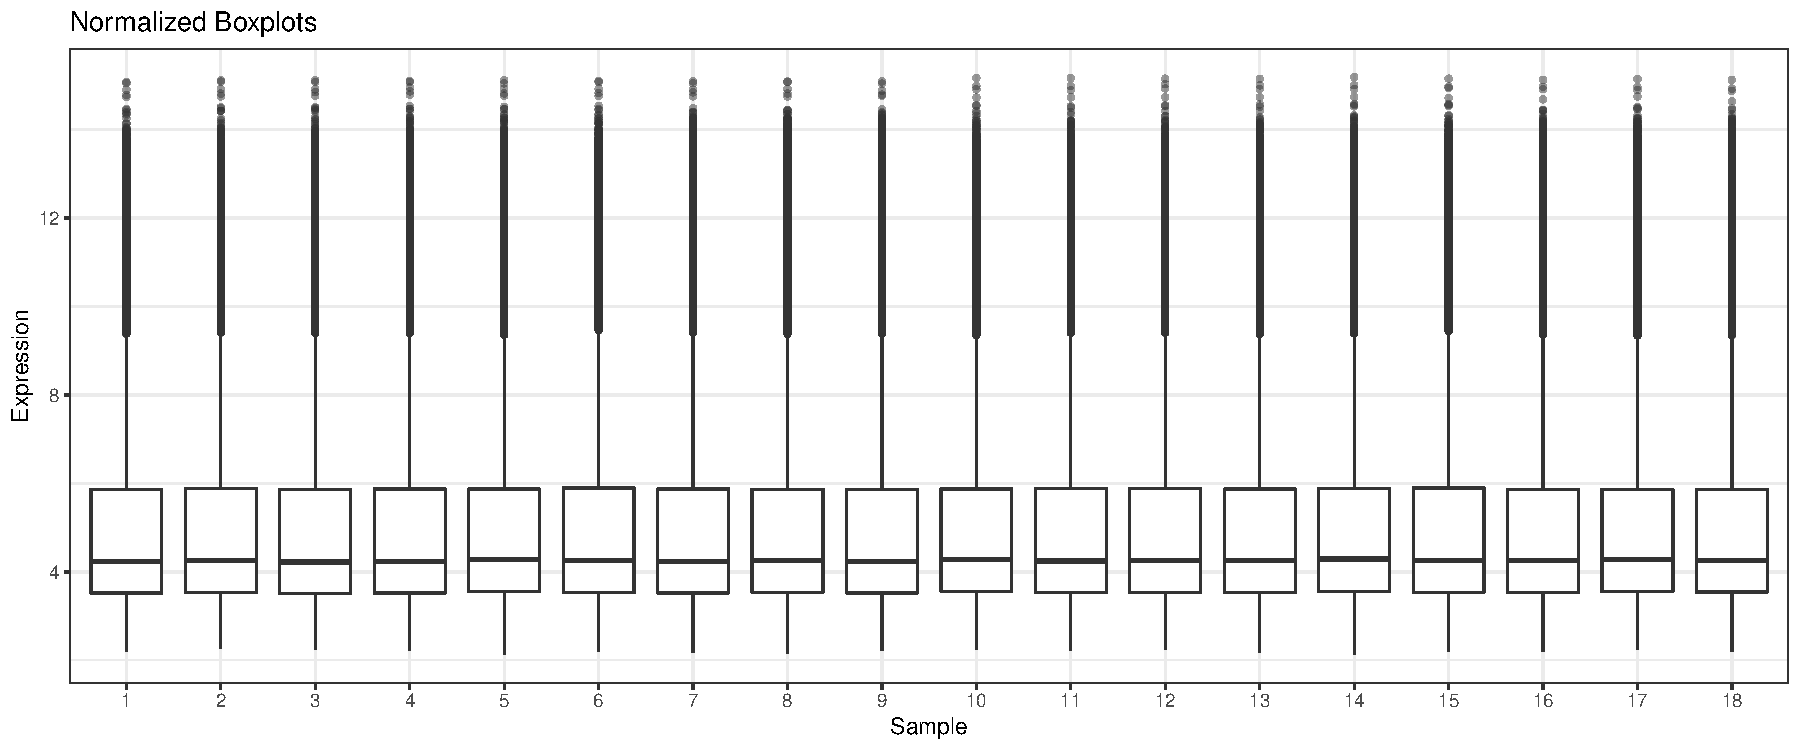
\includegraphics{resources/images/Normalized Boxplots.pdf}
    \caption{Normalized expression boxplot. This plot was generated with the \mono{prepaffy} command on the spike-in Data from \textcite{zhuPreferredAnalysisMethods2010}. Each boxplot refers to a sample. The boxplots are numbered, and are in the same order as the input files.}
    \label{fig:ExprBoxplot}
\end{figure}

\subsection{Dendrogram, PCA and Scree plots}
Hierarchical clustering dendrograms (hereby referred to as "dendrograms"), \gls{pca} plots and Scree plots allow the visual detection of clustering of the data.

Dendrograms show the hierarchical distances between the samples. Samples connected more closely than others are more clustered. An example of such a plot can be seen in Figure \ref{fig:ClusterDendro}.

\begin{figure}
    \centering
    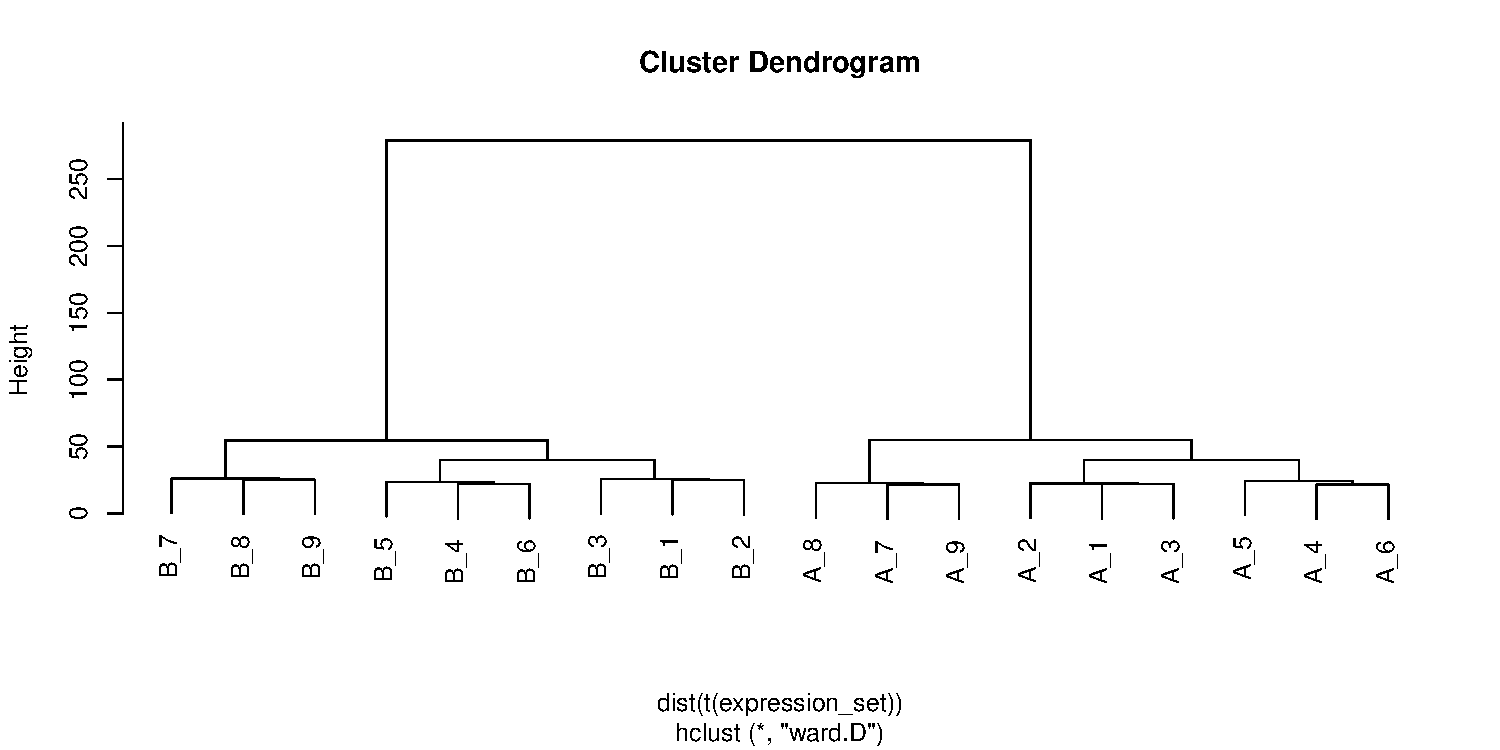
\includegraphics{resources/images/4_Dendrogram - original.pdf}
    \caption{A hierarchical clustering dendrogram plot of spike-in data from \textcite{zhuPreferredAnalysisMethods2010}. The data shows very large distances between the "A" and "B" samples, with smaller distances inside each group.}
    \label{fig:ClusterDendro}
\end{figure}

\gls{pca} plots show the result of the \gls{pca} analysis of the data. The main \gls{pca} plot shows principal component 1 vs principal component 2 of the samples. An example of such a plot can be seen in Figure \ref{fig:PCAplot}. An additional collection of \gls{pca} plots, named "PCA pairs", can also be found, and show plots generated from the combinations of other principal components.

\begin{figure}
    \centering
    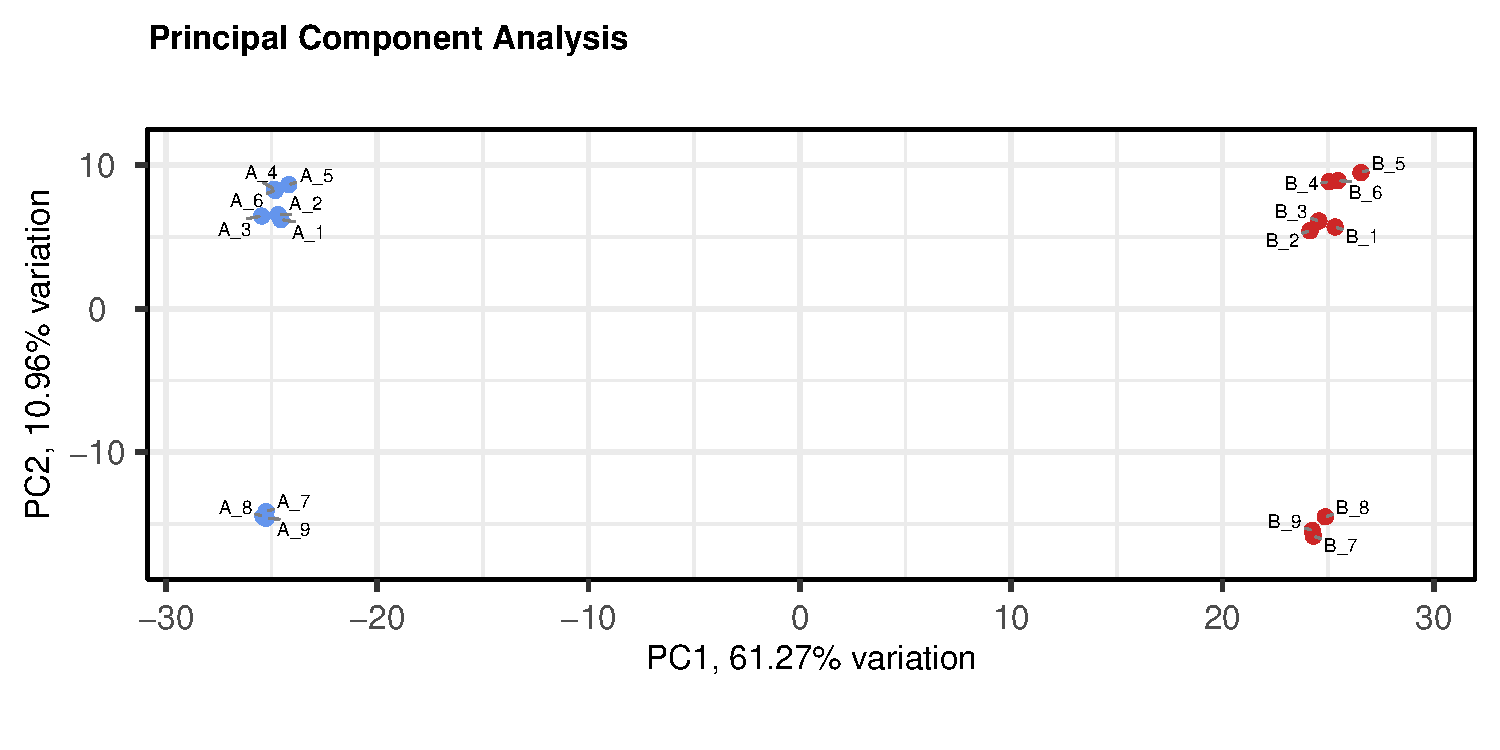
\includegraphics{resources/images/6_PCA - original.pdf}
    \caption{PCA plot of spike-in data from \textcite{zhuPreferredAnalysisMethods2010}. The data shows similar clustering as in Figure \ref{fig:ClusterDendro}, however, additional batch effects become clearer inside the two sample types.}
    \label{fig:PCAplot}
\end{figure}

Closely associated with the \gls{pca} plots is the Scree plot. The Scree plot shows the variability captured by each principal component, as well as the rolling sum of the captured variability. An example Scree plot can be seen in Figure \ref{fig:Scree}. It is useful to consider the Scree plot together with the \gls{pca} plots. If principal components cannot capture most of the variability of the data, the \gls{pca} plots are less informative.

\begin{figure}
    \centering
    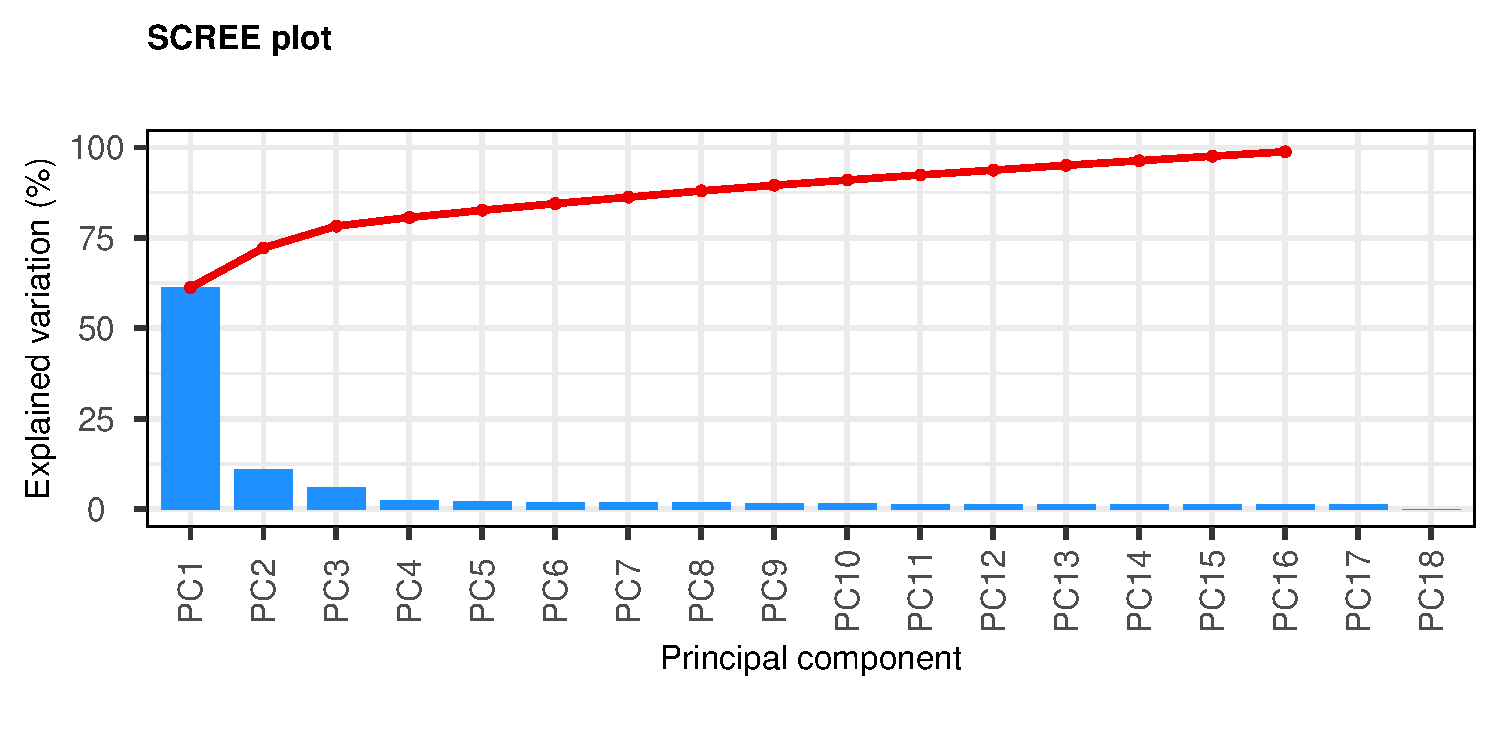
\includegraphics{resources/images/5_Scree Plot - original.pdf}
    \caption{Scree plot of spike-in data from \textcite{zhuPreferredAnalysisMethods2010}. As the first principal component captures most of the variability of the data, the \gls{pca} plots are very informative.}
    \label{fig:Scree}
\end{figure}

We expect the samples to be homogeneously distant from each other, with any obvious clustering a sign of a possible batch effect. The main exception from this rule of thumb is the clustering of different types of samples, for instance between the conditions of interest. While such a clustering (especially if very dramatic) could be due to batch effects that are not of interest, they could be a sign of important effects of the actual conditions. Therefore, light clustering of samples with the same conditions of interest can be normal.

\subsection{Poisson plots}
Poisson plots, or SD vs Mean plots, show the relationship between the standard deviation and the average of all genes in a certain group or groups. An example of such a plot can be seen in Figure \ref{fig:poissonplot}.

\begin{figure}
    \centering
    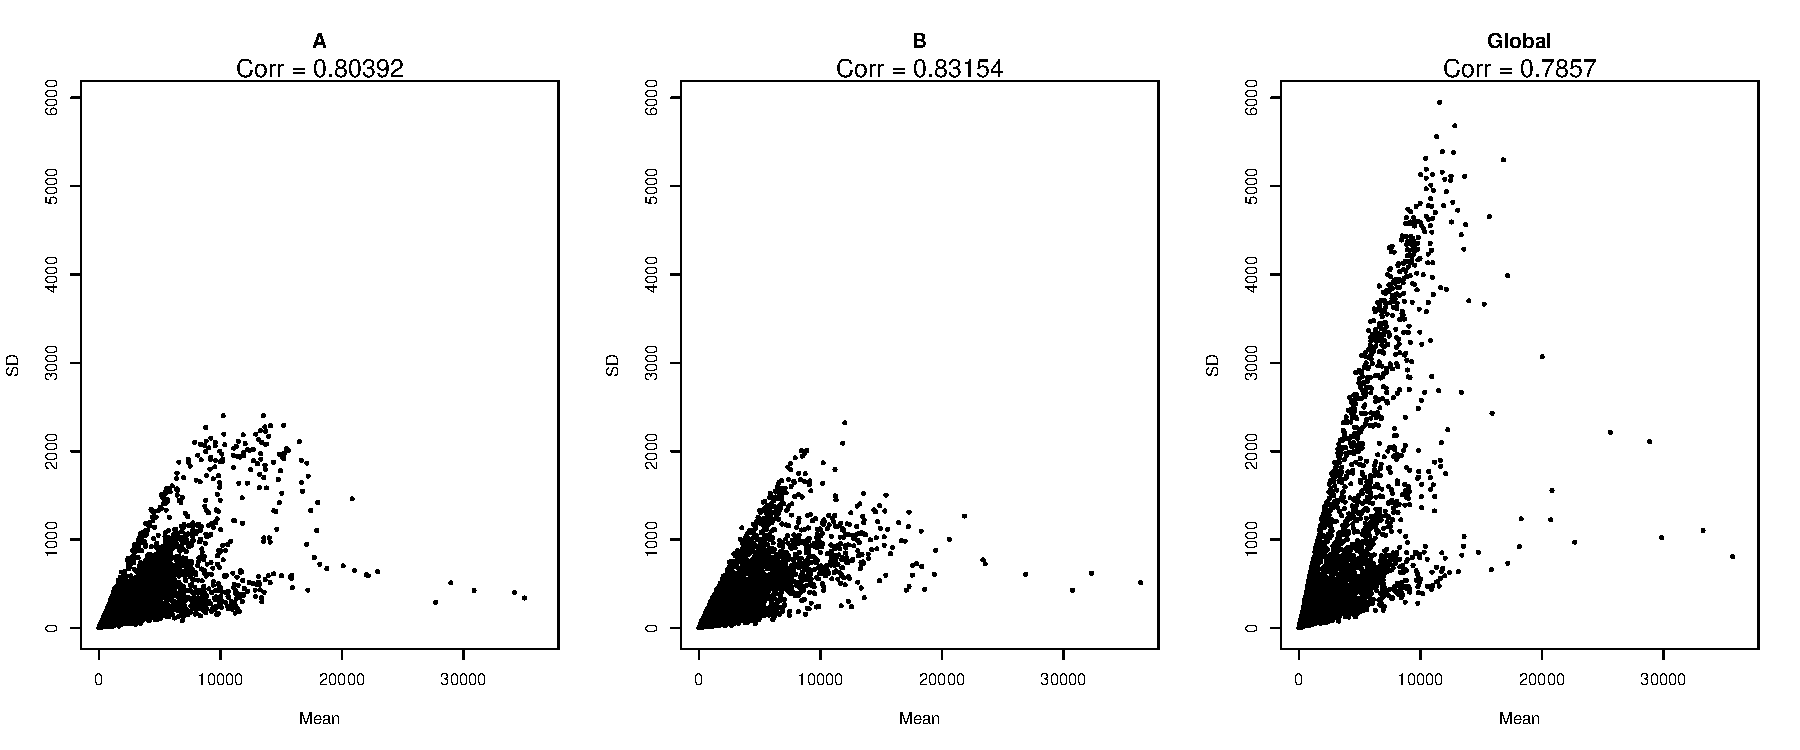
\includegraphics{resources/images/12_SD_vs_Mean Plot.pdf}
    \caption{A Poisson plot generated from the spike-in data from \textcite{zhuPreferredAnalysisMethods2010}. As expected, the data is roughly Poissonian, that is, the standard deviation is positively correlated with the mean. The same plot is drawn for the samples of condition "A", condition "B", and the summary of all samples ("Global").}
    \label{fig:poissonplot}
\end{figure}

The data is expected to be roughly Poissonian, with the standard deviation positively correlated with the mean. Any distortion or artifacts in these plots could be symptoms of deeper problems in the array hybridization, exposure, or both. The specific problem should be identifiable from the other quality-control plots.

\subsection{Volcano Plots}
Volcano plots are useful to show the result of a \gls{dea}. The $Y$ axis shows the p-values associated to each gene in a certain contrast (such as group "B" vs group "A"), but in $\log_{10}$ scale, to allow a wide range of p-values to be plotted. The $X$ axis shows the respective $\log_2$ fold-changes of each gene.

Threshold lines are drawn on the plot: an horizontal line representing the p-value threshold for statistical significance, and two vertical lines showing the $\log_2$ fold change thresholds to be considered \glspl{deg}. Therefore, all genes that fall on the upper-left and upper-right quadrants are downregulated and upregulated \glspl{deg}, respectively.

Do note that the $Y$ axis shows P-values, which are not corrected for multiple hypothesis testing. It is the P-value threshold that is moderated, instead, so the highlighted genes are the same ones that would be shown by plotting \gls{fdr} or \gls{pfp} values on the $Y$ axis and using a threshold of $0.05$. The only difference is graphical: P-values show the genes as more spread-out, while corrected values are squashed.

\begin{figure}
    \centering
    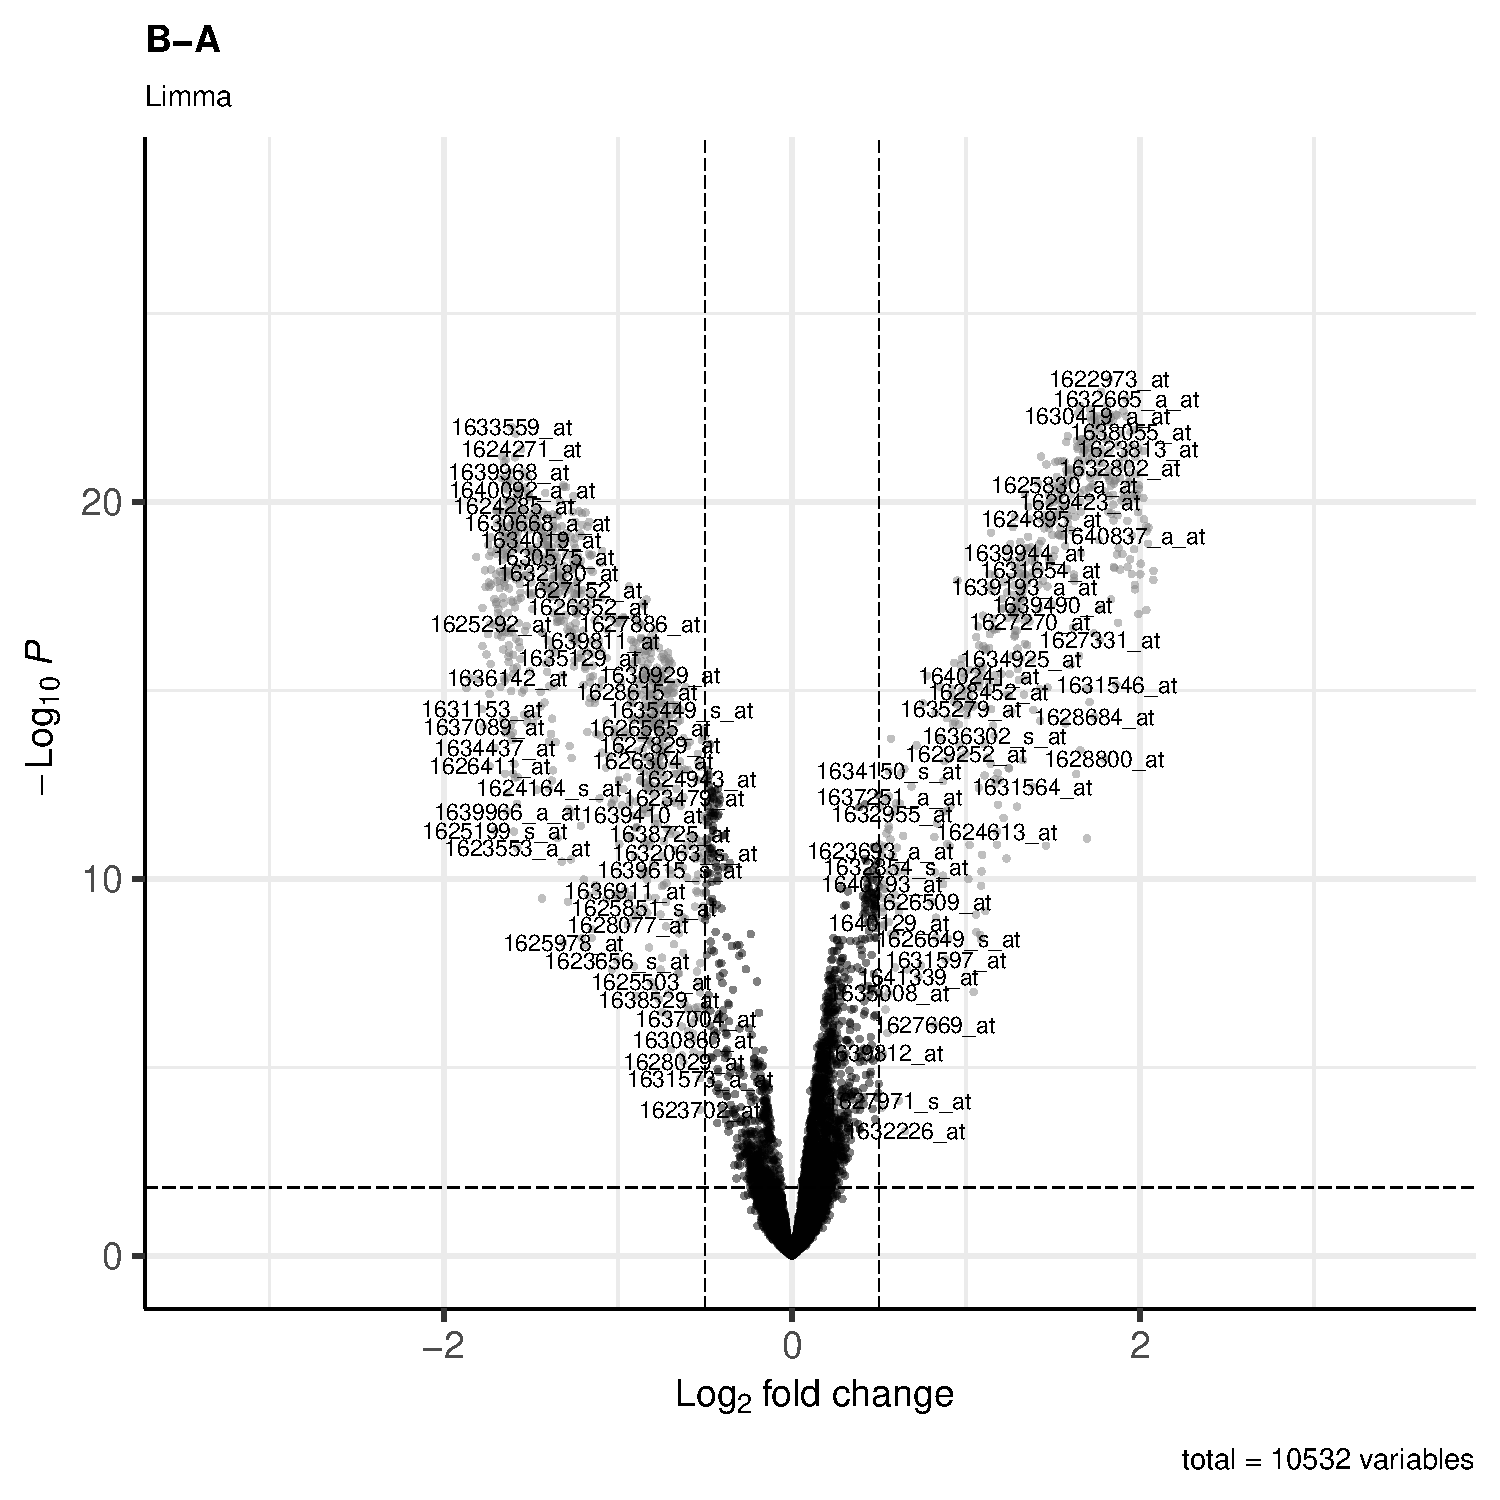
\includegraphics[width=0.85\textwidth]{resources/images/15_Volcano with Limma DEGs B-A.pdf}
    \caption{Volcano plot of the results of the \mono{limma} analysis on the spike-in dataset from \textcite{zhuPreferredAnalysisMethods2010}. The lower horizontal dotted line represents the corrected p-value equal to an \gls{fdr} threshold of $0.05$. The vertical lines represent the $\log_2$ fold change threshold of the analysis. The genes in the upper-left and upper-right quadrants are downregulated and upregulated \glspl{deg}, respectively.}
    \label{fig:volcanolimma}
\end{figure}

Volcano plots created by \gls{gattaca} can be labelled with \gls{hugo} symbols, if an annotation database is specified when calling \mono{gattaca run}. If unspecified, the probe ids are used instead (as seen in Figure \ref{fig:volcanolimma}).


\section{Computational reproducibility}
\gls{gattaca} allows the investigators to easily achieve computational reproducibility. Only a few items have to be recorded (and shared) to allow an identical run even far in the future. These are:
\begin{itemize}
    \item Any input files;
    \item The version of the docker used;
    \item For \mono{prepaffy} and \mono{prepagil}, it is sufficient to save the call to the tool.
    \item For \mono{run}, recording the options file used in the analysis is sufficient to reproduce it identically. In this case, the call to the tool has no influence to the run.
    \item For \mono{annotate}, it is sufficient to save the call to the tool.
\end{itemize}

\section{Install and use GATTACA interactively}
\label{localGATTA}
\gls{gattaca} is not distributed as a standalone package on CRAN. However, it could be useful in more complex analyses to access its functions directly in a non-dockerized environment. To do this, clone the repository locally (you must have \mono{git} installed):
\begin{lstlisting}
git clone https://github.com/Feat-FeAR/GATTACA.git
\end{lstlisting}
This will clone the repository locally into a new \mono{GATTACA/} folder. Copy the \mono{GATTACA/src} folder in your own project. Install the dependencies needed by \gls{gattaca} in your local R installation or virtual environment by \href{https://github.com/Feat-FeAR/GATTACA/blob/main/CONTRIBUTING.md}{following the CONTRIBUTING.md guide} on GitHub. Finally, start R, change your working directory to be inside of the folder that contains \mono{src/} (such as inside \mono{../src}), and source the \mono{src/\_\_init\_\_.R} file before starting the analysis.
Afterwards, you may source any other module at will, calling \gls{gattaca} functions interactively. Refer to the various help messages and comments in the source code for additional help.

\subsection{Contributing}

The same steps can be used to contribute to \gls{gattaca}. For more information, refer to \href{https://github.com/Feat-FeAR/GATTACA/blob/main/CONTRIBUTING.md}{the CONTRIBUTING.md guide} on GitHub. Every contribution is welcome.

The \href{https://github.com/Feat-FeAR/GATTACA/issues}{GitHub issues page} has information on the current issues and improvements that require contributions.
